%{ \setbeamercolor{frametitle}{fg=black,bg=black}
%\begin{frame} [fragile] 
%\frametitle{Messaggio ICMP Parameter Problem} 
%\begin{bytefield}[bitwidth=\linewidth/32]{32} 
%    \bitheader{0-31} \\
%    \bitbox{8}{Type} & \bitbox{8}{Code} & \bitbox{16}{Checksum} \\
%    \bitbox{8}{\textbf{\textcolor{purple}{Pointer}}} & \bitbox{24}{\textcolor{purple}{\textbf{Unused}}} \\
%    \bitbox{32}{\textcolor{purple}{\textbf{Internet Header+64 bits} of Original Datagram}} \\
%\end{bytefield}
%Inviato quando in un pacchetto si trova un problema con i parametri dell'intestazione. 
%%In modo tale da non poter completare l'elaborazione del datagramma. 
%\end{frame} }

\setbeamercolor{frametitle}{fg=black,bg=black}
\begin{frame}
\frametitle{Inserimento nel \textcolor{magenta}{campo Pointer} e \textcolor{magenta}{Unused}} 
\begin{columns}[T,onlytextwidth]
\column{0.48\textwidth} 
%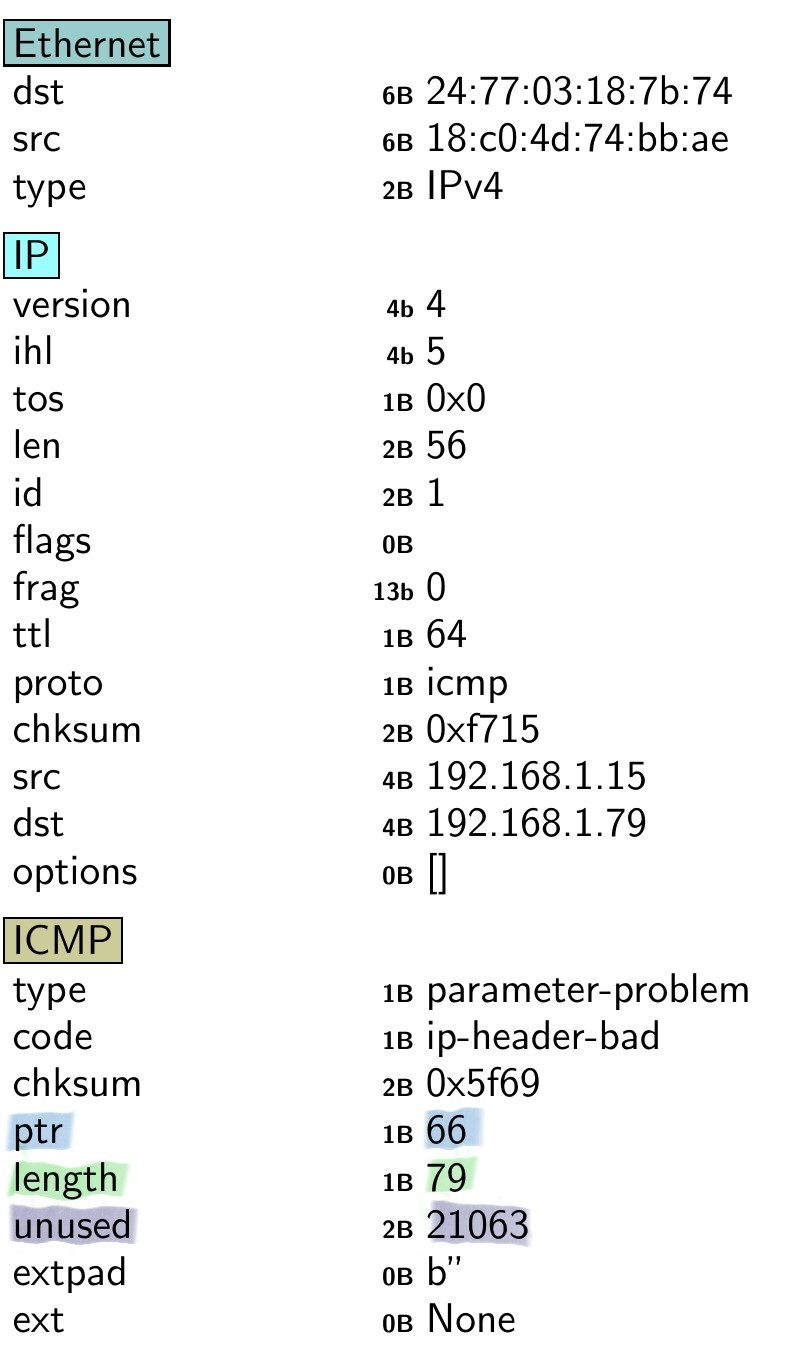
\includegraphics[width=0.45\textwidth]{../Tesi/img/ICMP_storageCC/parameterproblem_unused1_msg1.jpeg}
%\\
%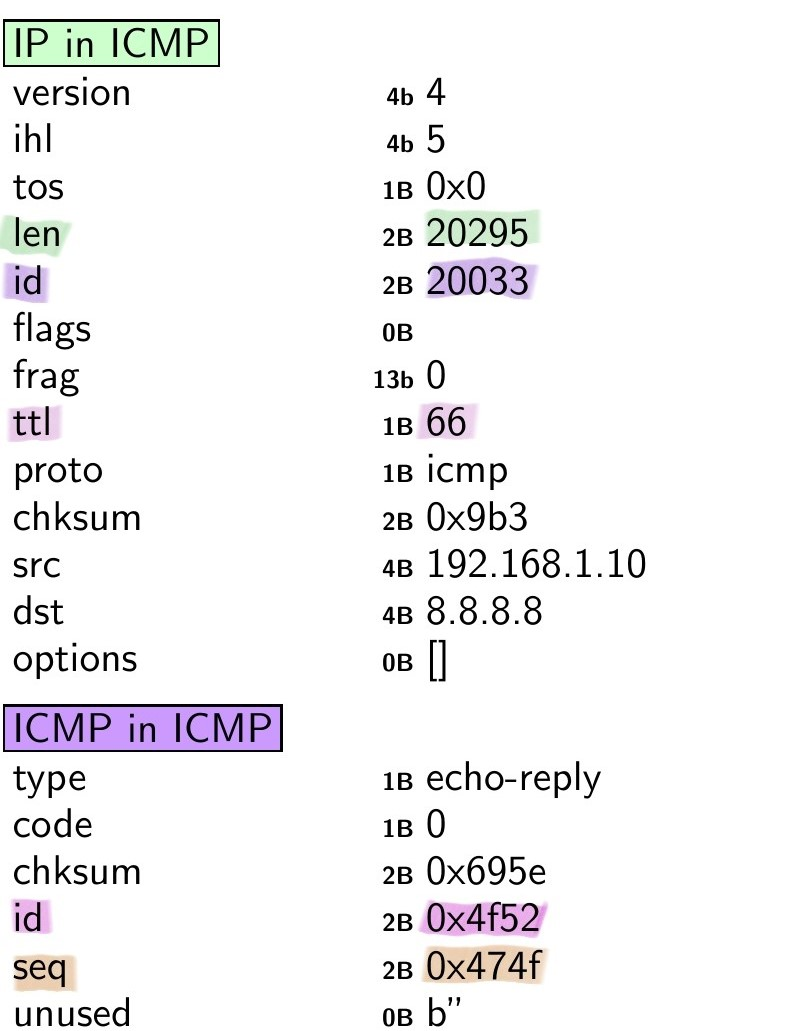
\includegraphics[width=0.45\textwidth]{../Tesi/img/ICMP_storageCC/parameterproblem_unused1_msg2.jpeg}
\vspace{1em} 
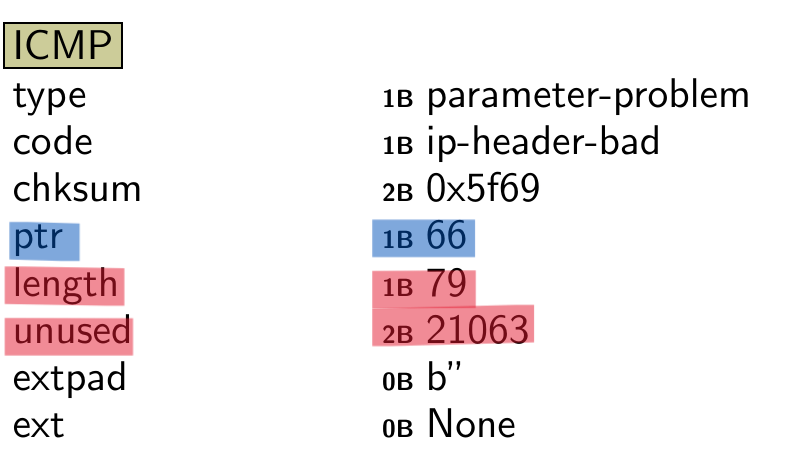
\includegraphics[width=\textwidth]{../Tesi/img/ICMP_storageCC/parameterproblem_unused1_msg_icmp_IP_ext.png}
%\captionof{figure}{Messaggio ICMP Parameter Problem}
\column{0.48\textwidth} 
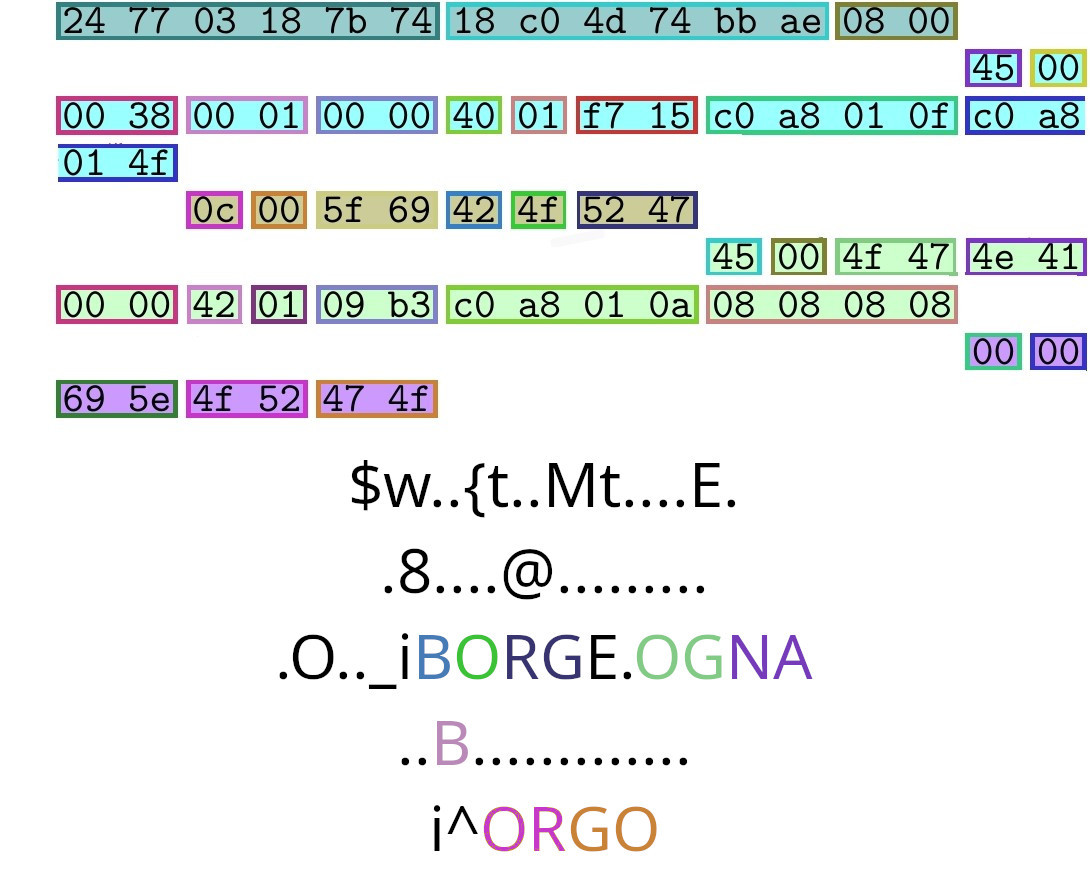
\includegraphics[width=\textwidth]{../Tesi/img/ICMP_storageCC/parameterproblem_unused1_hex.jpeg}
%\captionof{figure}{Dump esadecimale del messaggio}
\end{columns} 
\end{frame}


\begin{frame} [fragile] 
\frametitle{Inserimento nel \textcolor{magenta}{campo Internet Header+64 bits}}
%\begin{figure}  
%\centering
\scriptsize
\begin{bytefield}[bitwidth=\linewidth/32]{32}  
    \bitbox[]{32}{\textbf{IPv4 Header}} \\
    \bitheader{0-31} \\
    \bitbox{4}{Version} & \bitbox{4}{IHL} & \bitbox{8}{Type of Service} & \bitbox{16}{\textbf{\textcolor{purple}{Total Length}}} \\
    \bitbox{16}{\textbf{\textcolor{purple}{Identification}}} & \bitbox{3}{Flags} & \bitbox{13}{Fragments Offset} \\
    \bitbox{8}{\textbf{\textcolor{purple}{Time to Live}}} & \bitbox{8}{Protocol} & \bitbox{16}{Header Checksum} \\
    \bitbox{32}{Source Address} \\
    \bitbox{32}{Destination Address} \\
    %\bitbox{24}{Options} & \bitbox{8}{Padding} \\[0.3em]
    \bitbox[]{32}{\textbf{First 64 bits}} \\
    \bitheader{0-31} \\
    \bitbox{8}{Type} & \bitbox{8}{Code} & \bitbox{16}{Checksum} \\
    \bitbox{16}{\textbf{\textcolor{purple}{Identifier}}} & \bitbox{16}{\textbf{\textcolor{purple}{Sequence Number}}} \\
\end{bytefield}
%\captionof{figure}{Struttura del campo \textit{Header+64 bits}}
%\end{figure} 
\end{frame} 

\begin{frame} 
\begin{columns}[T,onlytextwidth]
\column{0.48\textwidth} 
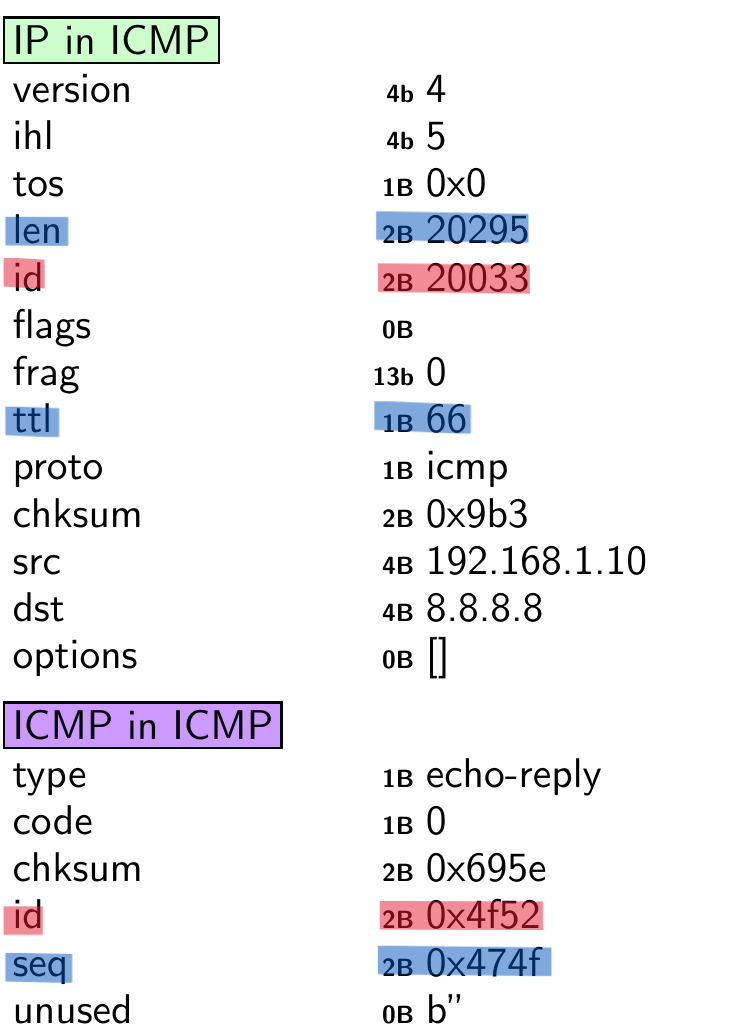
\includegraphics[width=\textwidth]{../Tesi/img/ICMP_storageCC/immagie_header_64bit_ICMP.png}
%\captionof{figure}{Contenuto di \textit{Header+64 bits}}
\column{0.48\textwidth} 
\vspace{10ex} 
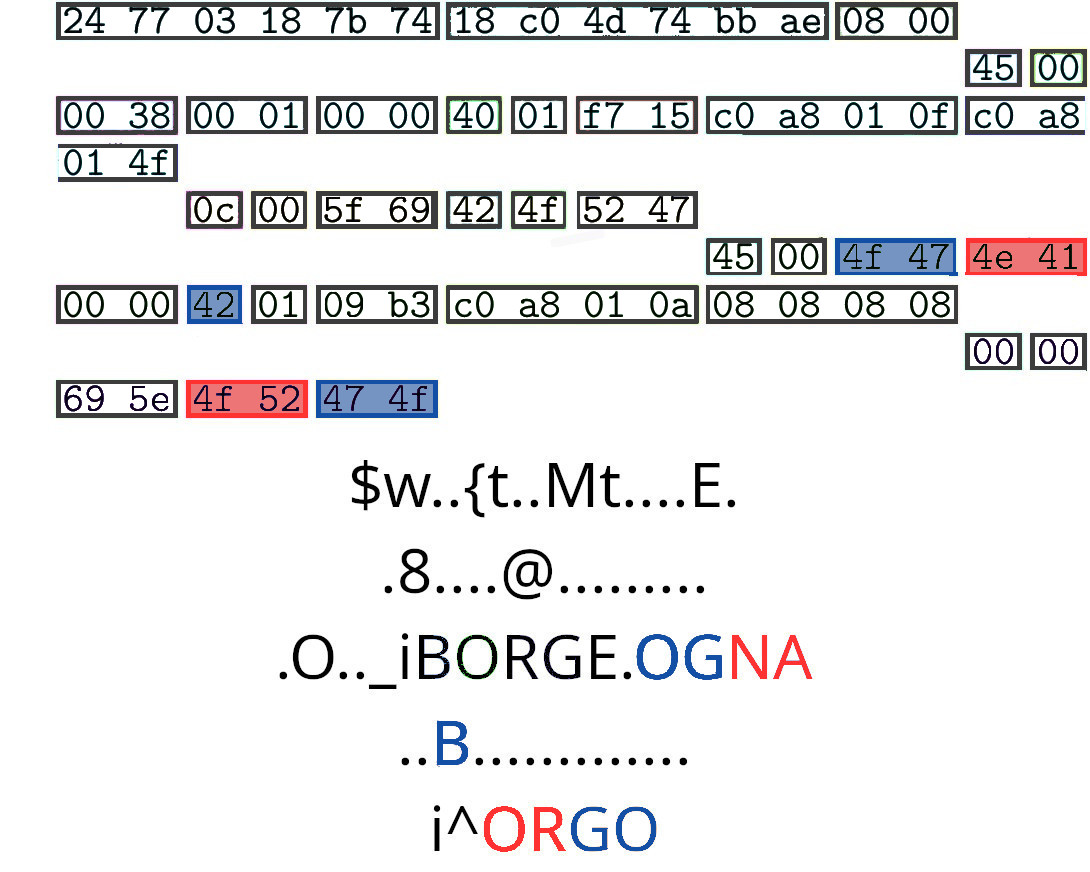
\includegraphics[width=0.9\textwidth]{../Tesi/img/ICMP_storageCC/immagie_header_64bit_hex.jpeg}
%\captionof{figure}{Dump esadecimale del messaggio}
%\scriptsize
%\begin{longtable}{|p{0.4\textwidth}|p{0.4\textwidth}|} 
%    \multicolumn{2}{c}{Header IPv4} \\ \hline 
%    \textbf{Campo} & \textbf{Byte} \\ \hline 
%    \textcolor{blue}{Total length} & 2 byte \\ \hline
%    \textcolor{red}{Identification} & 2 byte \\ \hline 
%    \textcolor{blue}{Time to live} & 1 byte \\ \hline 
%    \noalign{\vskip 2ex}
%    \multicolumn{2}{c}{Header ICMPv4} \\ \hline
%    \textbf{Campo} & \textbf{Byte} \\ \hline 
%    \textcolor{red}{Identifier} & 2 byte \\ \hline 
%    \textcolor{blue}{Sequence} & 2 byte \\ \hline
%    %\caption{Uso del Header+64 bits nel caso di IP/ICMP} 
%\end{longtable}  
\end{columns} 
\end{frame} 

%{\setbeamercolor{frametitle}{fg=black,bg=black}
%\begin{frame} [fragile] 
%\frametitle{Messaggio ICMP Echo Request/Reply} 
%\begin{bytefield}[bitwidth=\linewidth/32]{32} 
%    \bitheader{0-31} \\
%    \bitbox{8}{Type} & \bitbox{8}{Code} & \bitbox{16}{Checksum} \\
%    \bitbox{16}{\textbf{\textcolor{purple}{Identifier}}} & \bitbox{16}{Sequence Number} \\
%    \bitbox{32}{\textbf{\textcolor{purple}{Data}}} \\
%\end{bytefield} 
%Usato per determinare se un host è connesso.
%\end{frame} }

\begin{frame} 
\frametitle{Inserimento nel \textcolor{magenta}{campo Identifier}} 
\begin{columns}[T,onlytextwidth] 
\column{0.48\textwidth}  
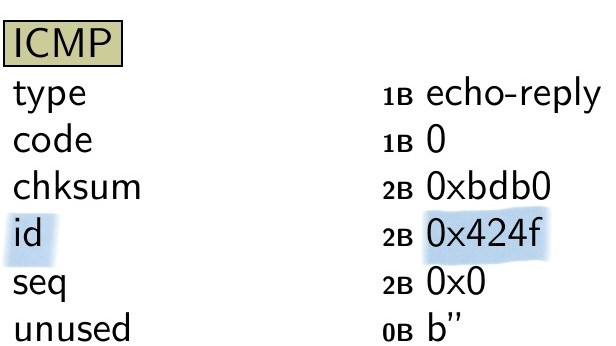
\includegraphics[width=0.8\textwidth]{../Tesi/img/ICMP_storageCC/packet_echo_identifier1_msg_icmp.jpeg}
\captionof{figure}{1° messaggio ICMP Echo Reply}
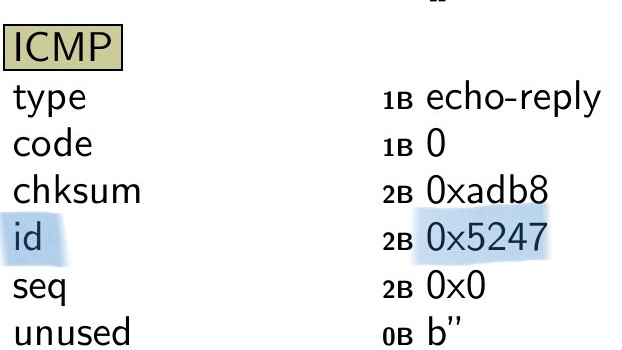
\includegraphics[width=0.8\textwidth]{../Tesi/img/ICMP_storageCC/packet_echo_identifier2_msg_icmp.jpeg}
\captionof{figure}{2° messaggio ICMP Echo Reply}
\column{0.48\textwidth}  
\vspace{1ex} 
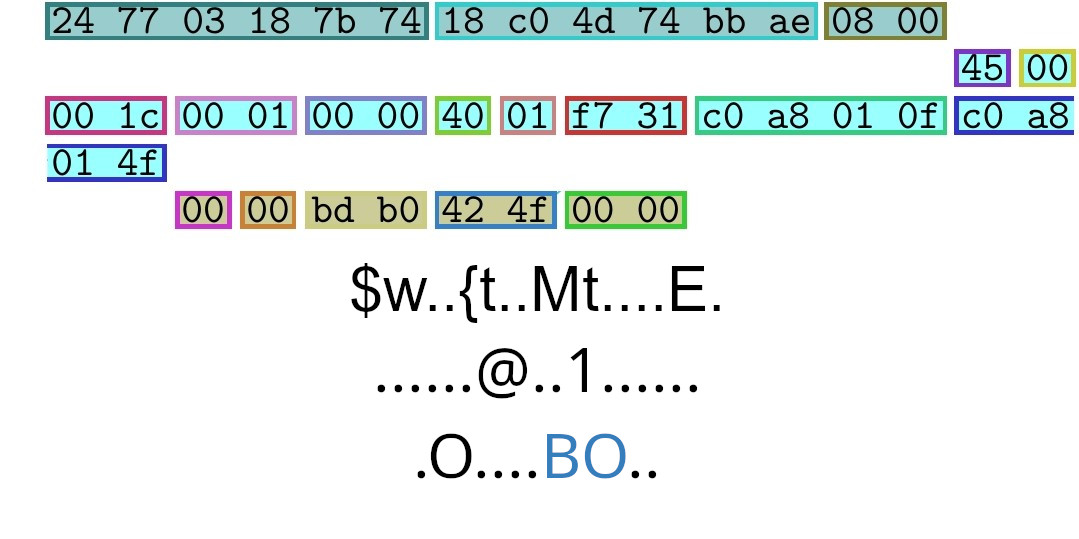
\includegraphics[width=\textwidth]{../Tesi/img/ICMP_storageCC/packet_echo_identifier1_hex_testo.jpeg}
%\captionof{figure}{Dump esadecimale del messaggio}
\vspace{2ex} \newline
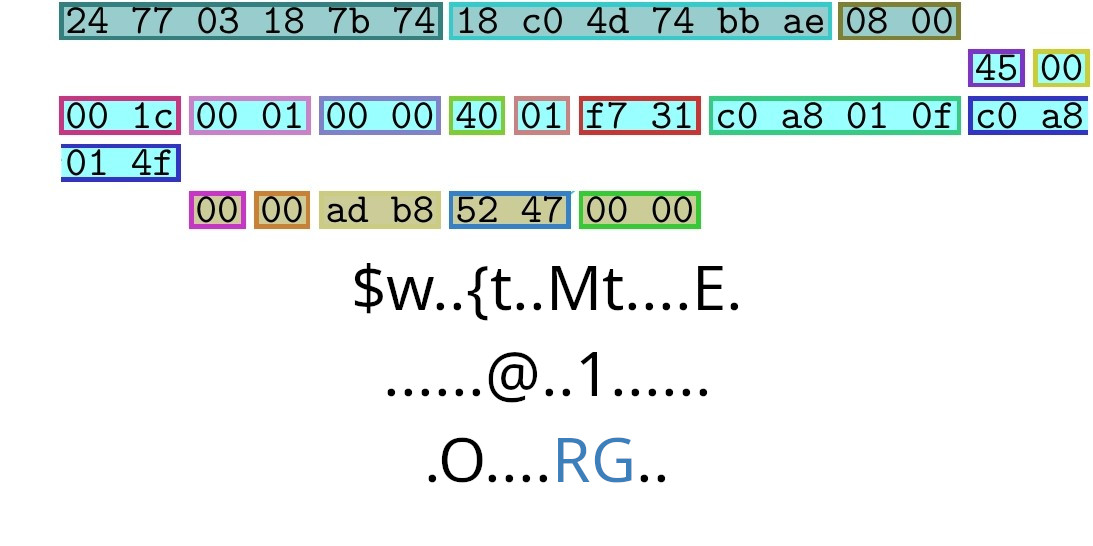
\includegraphics[width=\textwidth]{../Tesi/img/ICMP_storageCC/packet_echo_identifier2_hex_testo.jpeg}
%\captionof{figure}{Dump esadecimale del messaggio}
\end{columns} 
\end{frame} 

%\begin{frame}[fragile] %allowframebreaks
%\begin{columns}[T,onlytextwidth]
%\column{0.48\textwidth}  
%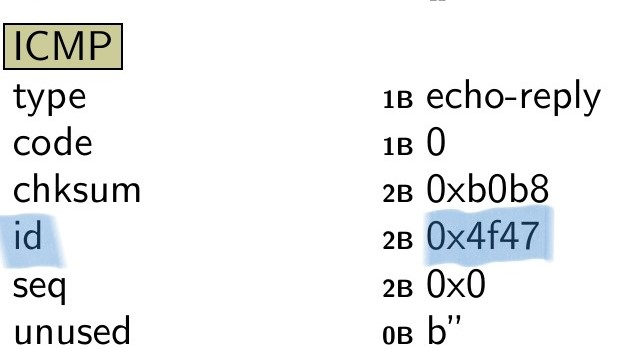
\includegraphics[width=0.8\textwidth]{../Tesi/img/ICMP_storageCC/packet_echo_identifier3_msg_icmp.jpeg}
%\captionof{figure}{3° messaggio ICMP Echo Reply}
%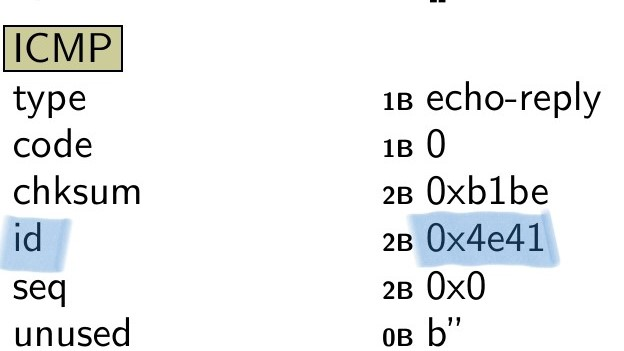
\includegraphics[width=0.8\textwidth]{../Tesi/img/ICMP_storageCC/packet_echo_identifier4_msg_icmp.jpeg}  
%\captionof{figure}{4° messaggio ICMP Echo Reply}
%\column{0.48\textwidth}  
%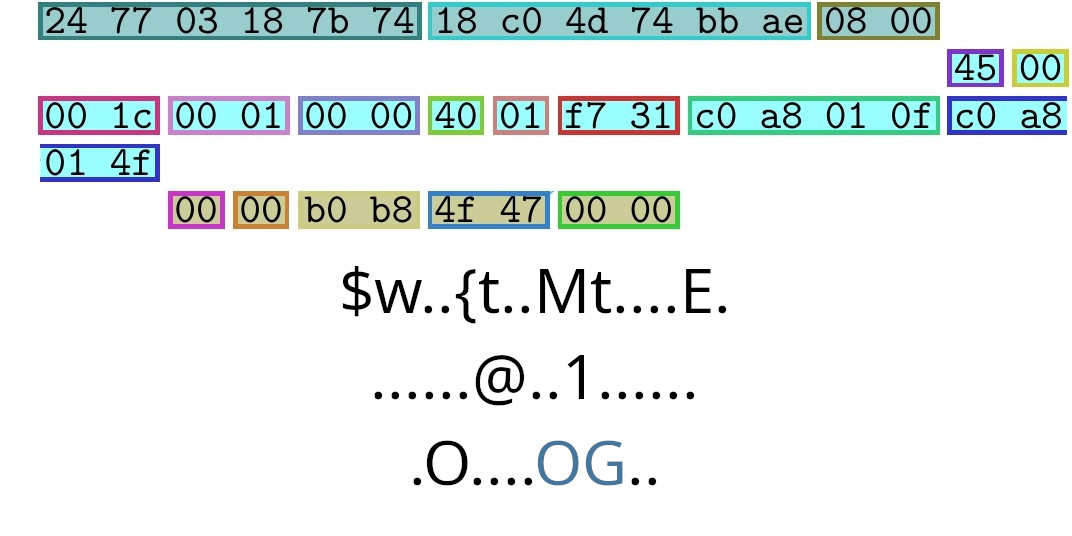
\includegraphics[width=0.8\textwidth]{../Tesi/img/ICMP_storageCC/packet_echo_identifier3_hex_testo.jpeg}
%\captionof{figure}{Dump esadecimale del messaggio}
%\vspace{4ex}
%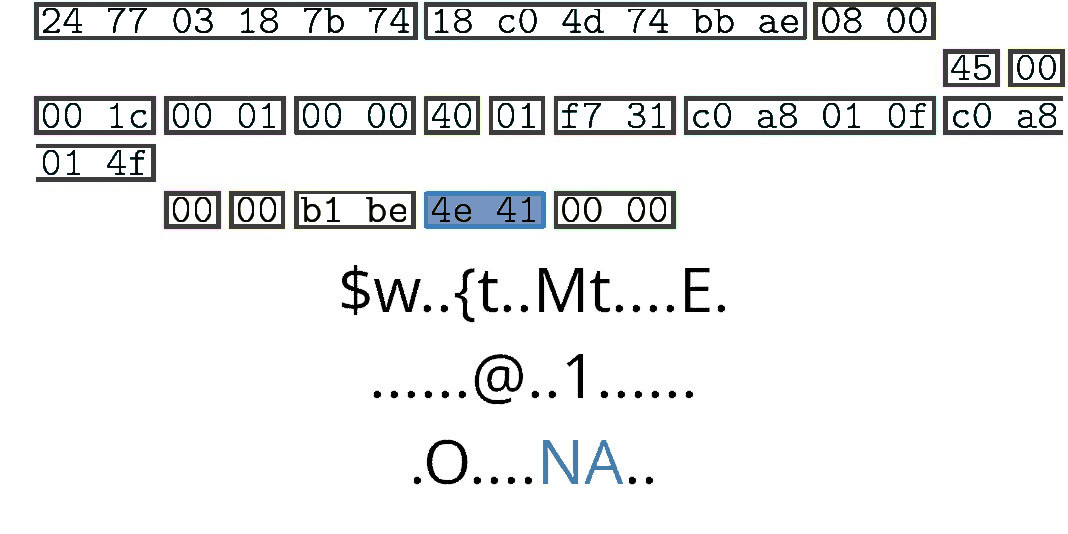
\includegraphics[width=0.8\textwidth]{../Tesi/img/ICMP_storageCC/packet_echo_identifier4_hex_testo.jpeg}
%\captionof{figure}{Dump esadecimale del messaggio}
%\end{columns} 
%\end{frame} 

\begin{frame} 
\frametitle{Inserimento nel \textcolor{magenta}{campo Data}} 
\begin{columns}[T,onlytextwidth]
\column{0.48\textwidth}  
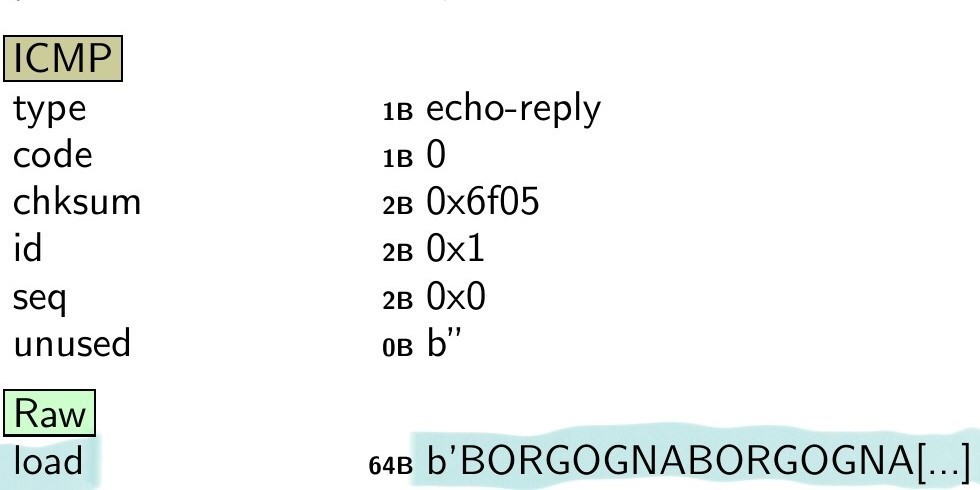
\includegraphics[width=\textwidth]{../Tesi/img/ICMP_storageCC/packet_echo_payload_msg_icmp.jpeg}
%\captionof{figure}{Messaggio ICMP Echo Reply}
\column{0.48\textwidth} 
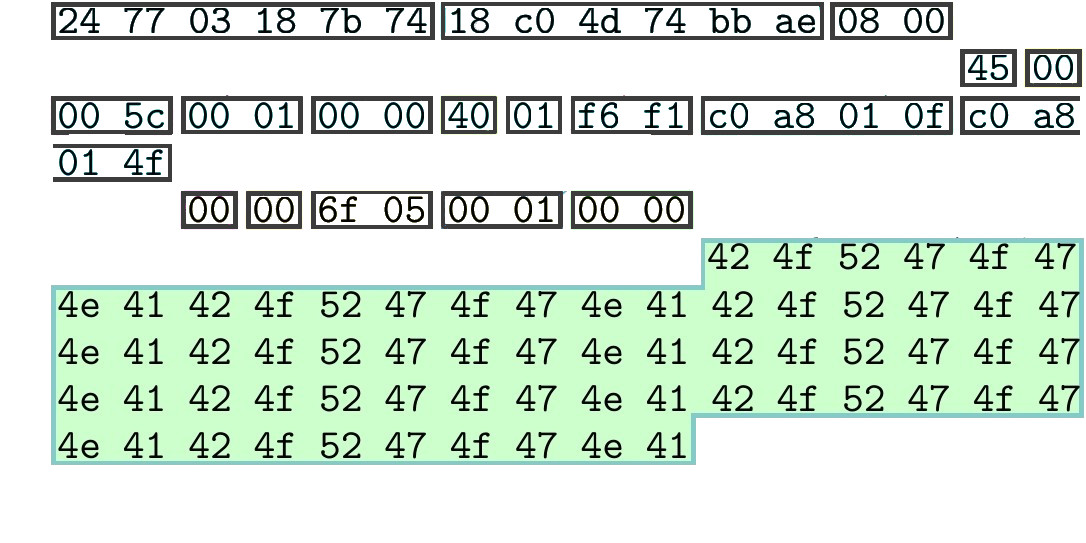
\includegraphics[width=\textwidth]{../Tesi/img/ICMP_storageCC/packet_echo_payload_hex.jpeg}
%\captionof{figure}{Dump esadecimale messaggio ICMP Echo Reply}
\end{columns}
\end{frame}  

%{\setbeamercolor{frametitle}{fg=black,bg=black}
%\begin{frame} [fragile] 
%\frametitle{Messaggio ICMP Timestamp Request/Reply} 
%\begin{bytefield}[bitwidth=\linewidth/32]{32} 
%    \bitheader{0-31} \\
%    \bitbox{8}{Type} & \bitbox{8}{Code} & \bitbox{16}{Checksum} \\
%    \bitbox{16}{\textbf{\textcolor{purple}{Identifier}}} & \bitbox{16}{Sequence Number} \\
%    \bitbox{32}{\textbf{\textcolor{purple}{Originate Timestamp}}} \\
%    \bitbox{32}{\textbf{\textcolor{purple}{Receive Timestamp}}} \\
%    \bitbox{32}{\textbf{\textcolor{purple}{Transmit Timestamp}}} \\
%%\bitbox{32}{Data ... ($\geq$ 0 byte)}  
%\end{bytefield} 
%Usato per misurare la sincronizzazione dei clock
%\end{frame} }

\begin{frame} 
\frametitle{Inserimento nel \textcolor{magenta}{campo Timestamp}} 
\begin{columns}[T,onlytextwidth]
\column{0.48\textwidth}   
\vspace{6ex}
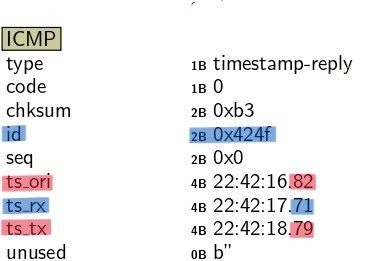
\includegraphics[width=0.9\textwidth]{../Tesi/img/ICMP_storageCC/timestamp_msg_icmp_milli.jpg}
%\captionof{figure}{Messaggio ICMP Timestamp} 
%\vspace{2ex}
%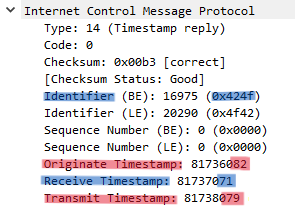
\includegraphics[width=0.9\textwidth]{../Tesi/img/ICMP_storageCC/timestamp_wireshark2_milli.PNG}
\column{0.48\textwidth}
\scriptsize
\begin{longtable}{|p{0.25\textwidth}|p{0.25\textwidth}|p{0.25\textwidth}|}  
    \hline 
    \textbf{Lettera} & \textbf{Hex} & \textbf{Dec} \\ \hline 
    B & \textcolor{blue}{42} & 66 \\ \hline
    0 & \textcolor{blue}{4F} & 79 \\ \hline  
    R & 52 & \textcolor{red}{82} \\ \hline
    G & 47 & \textcolor{blue}{71} \\ \hline
    O & 4F & \textcolor{red}{79} \\ \hline 
\end{longtable}  
%\captionof{figure}{Valore esadecimale e decimale dei caratteri ASCII}
\vspace{5ex}
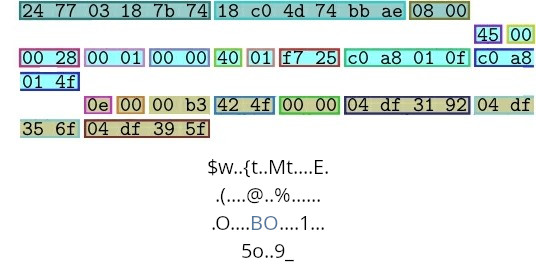
\includegraphics[width=\textwidth]{../Tesi/img/ICMP_storageCC/timestamp_hex.jpg}
%\captionof{figure}{Dump esadecimale messaggio ICMP Timestamp}
\end{columns}
\end{frame} 
